%% !TEX root = manual.tex

\section{SST/macro GUI}
\label{sec:basicgui}

The \sstmacro GUI is used for creating parameter files for an \sstmacro simulation, keeping track of which parameters are required
depending on the different models available.  See Section \ref{sec:building:gui} for instructions on building and running the GUI.


The GUI displays the various SST/macro components and sub-components as separate tabs.
\begin{center}
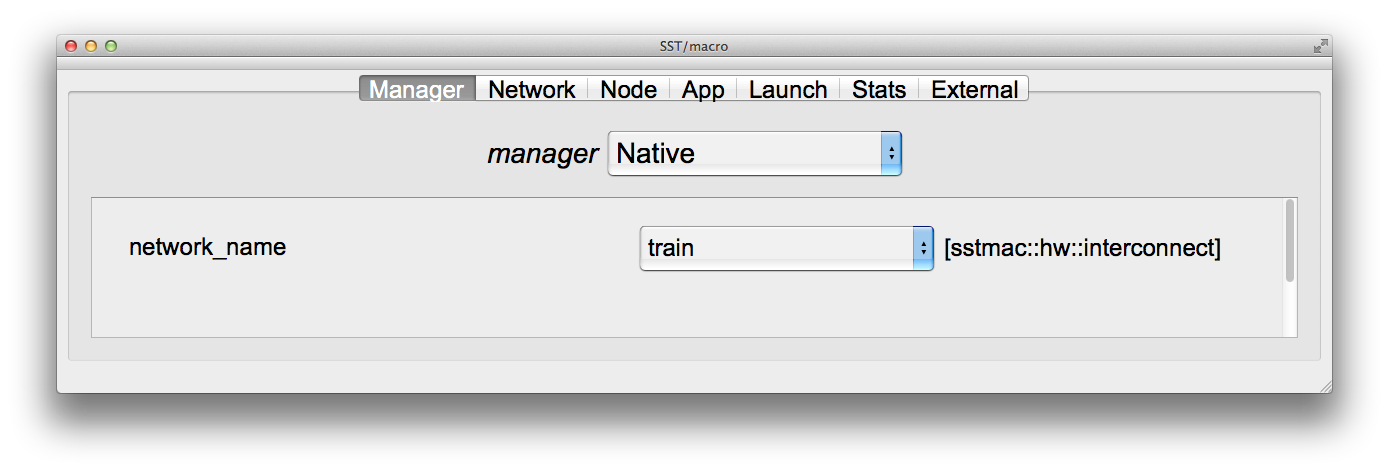
\includegraphics[width=1.0\textwidth]{figures/gui/manager.png}
\end{center}
The opening tab shows the discrete event manager. 
On the top, tabs for the major components can be seen such as the network, node, and the application.  
On the network tab, we have several subtabs for the various network components.
\begin{center}
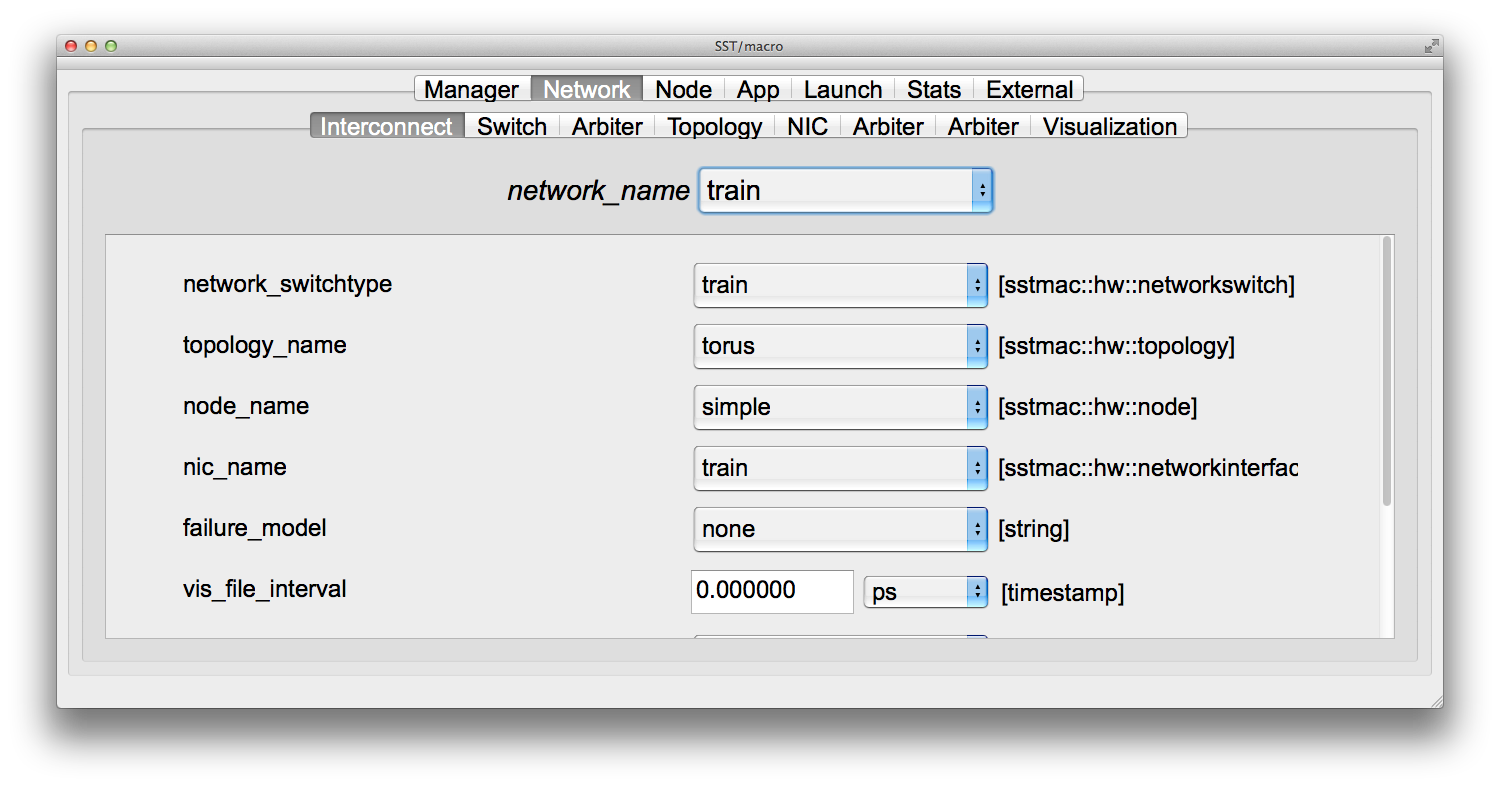
\includegraphics[width=1.0\textwidth]{figures/gui/network.png}
\end{center}
Here the most important tabs are interconnect, switch, topology, and NIC.   
We see the keyword \guikey{network\_switchtype} with value \guikey{train}.  
Most keywords are documented with tooltips to give a brief introduction to what each keyword means.
\begin{center}
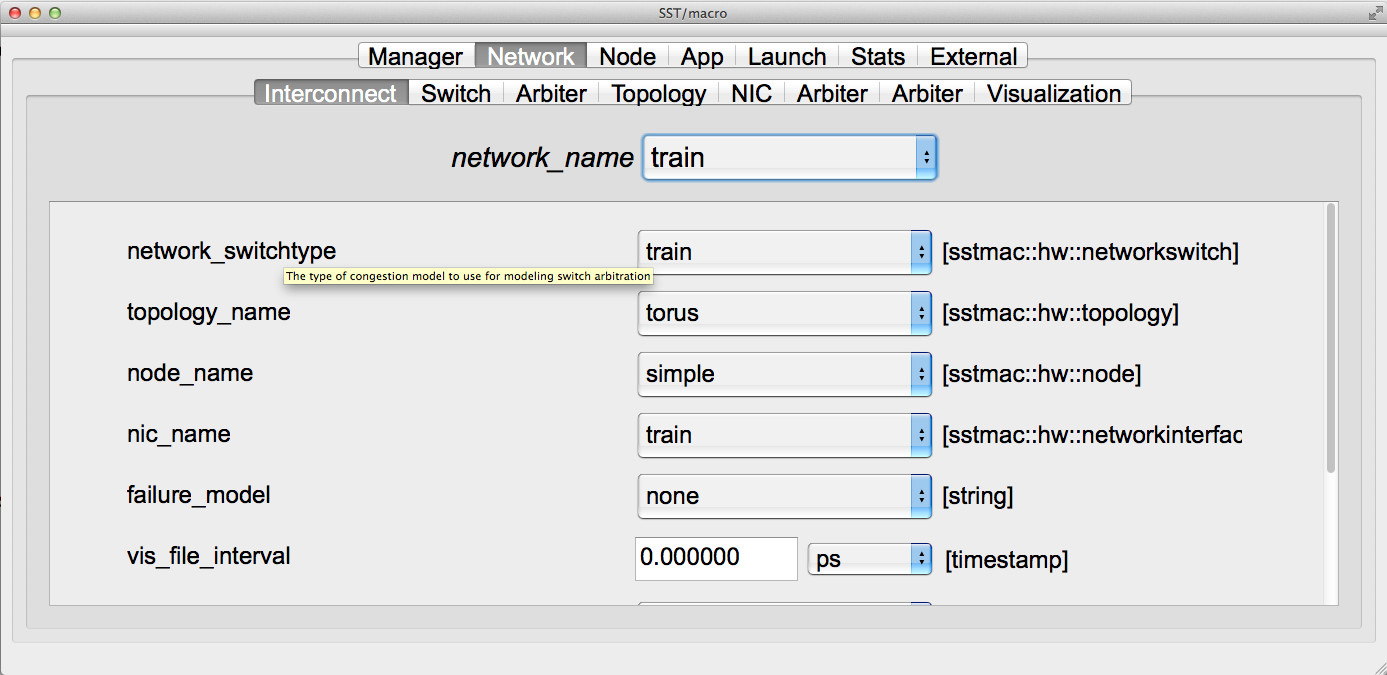
\includegraphics[width=1.0\textwidth]{figures/gui/networkswitchtooltip.png}
\end{center}
The tooltip indicates this keyword determines which model to use for simulating congestion in the network switches. 
The exact meaning of \guikey{train} is beyond the scope of this section (and the tooltip). 
For a brief introduction to congestion model, see \ref{sec:tutorial:networkmodel}.

At present, the GUI is only intended as a helper tool for constructing input files.  
Once a configuration is chosen, a parameter file can be generated by selecting File $\rightarrow$ Save and creating a \textit{.ini} file.  
Although a more comprehensive GUI is planned, experiments must still be run on the command line via parameter files.
